
\documentclass[border=10pt]{standalone}
\usepackage{pgfplots}
\pgfplotsset{compat=1.18}
\begin{document}
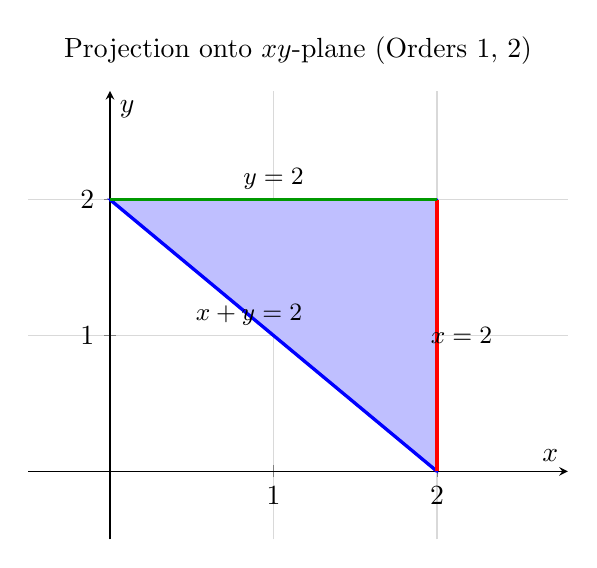
\begin{tikzpicture}
\begin{axis}[
    xmin=-0.5, xmax=2.8,
    ymin=-0.5, ymax=2.8,
    xlabel={$x$}, ylabel={$y$},
    title={Projection onto $xy$-plane (Orders 1, 2)},
    grid=major, grid style={gray!30},
    axis lines=middle,
    enlargelimits=false,
    xtick={0,1,2}, ytick={0,1,2},
]
% Filled triangle: (2,0), (0,2), (2,2)
\addplot[fill=blue!25, draw=blue, thick] coordinates {(2,0) (0,2) (2,2)} -- cycle;
% Boundary lines
\addplot[blue, very thick] coordinates {(2,0) (0,2)};
\node at (axis cs:0.85,1.15) {\small $x+y=2$};
\addplot[red, very thick] coordinates {(2,0) (2,2)};
\node at (axis cs:2.15,1.0) {\small $x=2$};
\addplot[green!60!black, very thick] coordinates {(0,2) (2,2)};
\node at (axis cs:1.0,2.15) {\small $y=2$};
\end{axis}
\end{tikzpicture}
\end{document}
